\documentclass[11pt]{article}

% Course rule (HW1 slides p.4): use [preprint] -- shows names and page numbers.
\usepackage[preprint]{acl}

\usepackage{times}
\usepackage{latexsym}
\usepackage[T1]{fontenc}
\usepackage[utf8]{inputenc}
\usepackage{microtype}
\usepackage{inconsolata}
\usepackage{graphicx}

% Chinese member names (works with pdfLaTeX, incl. Overleaf). bsmi = Traditional Chinese Ming font.
\usepackage{CJKutf8}
\newcommand{\zh}[1]{\begin{CJK}{UTF8}{bsmi}#1\end{CJK}}
% bsmi lacks the glyph for 瀞; take it from IPAex Mincho (ipaex-type1, in TeX Live / Overleaf).
\newcommand{\zhalt}[1]{\begin{CJK}{UTF8}{ipxm}#1\end{CJK}}

% Tables and math
\usepackage{booktabs}
\usepackage{array}
\usepackage{xurl}  % allow long URLs in the bibliography to break
\usepackage{multirow}
\usepackage{amsmath}
\usepackage{siunitx}

% Compact lists (item spacing only; margins and font size untouched).
\usepackage{enumitem}
\setlist[itemize]{noitemsep, topsep=2pt}

% Placeholder marker. Shows red text in the PDF so unfinished parts are easy to spot.
% Before submission: search for \todo and make sure none are left.
\usepackage{xcolor}
\newcommand{\todo}[1]{\textcolor{red}{[TODO: #1]}}

% ===================== Course requirements (HW1 slides) =====================
% - At most 6 pages EXCLUDING references. Pages after 6 are not read.
%   "Contributions of Each Member" counts toward the 6 pages.
% - Keep the template's margins and font size (no \vspace / font-size hacks).
% - Front matter: title, team ID, every member's name + student ID, GitHub URL.
%   No GitHub URL on page 1  =>  report scored 0.
% - Sections must appear in this order (titles may be adapted).
% - Figures/tables: numbered, captioned, referenced in text, axes with units.
% - Output file name on E3: HW1_<TeamID>_report.pdf
%
% Page budget (12 columns in total; roughly follows the section points):
%   Abstract + §1  ~1.25 col  (7 pts)    §5  ~1.5 col   (13 pts)
%   §2             ~1.0  col  (6 pts)    §6  ~1.0 col   (10 pts)
%   §3             ~1.5  col  (12 pts)   §7  ~1.75 col  (18 pts)
%   §4             ~1.25 col  (10 pts)   §8  ~1.75 col  (16 pts)
%   §9             ~0.5  col  (5 pts)    Contributions ~0.5 col (3 pts)
% ============================================================================

% Suggested title (discuss with the team):
%   Pricing Before the Sale: An Interpretable Elastic Net for Ames House Valuation
\title{Pricing Before the Sale: An Interpretable Elastic Net for Ames Houses}

\author{
  \textbf{Group 3} \\
  \zh{周懷聖} (315554046), \zh{范}\zhalt{瀞}\zh{予} (314554031), \zh{李宗穎} (312581021), \zh{劉嘉豪} (315552031),
\\
  \zh{張翊鞍} (314554035), \zh{陳柏淮} (315554045), \zh{陳家祥} (315552025)
\\
  \url{https://github.com/chouhuaishengcs15/Data-Mining-HW1}
}

\begin{document}
\maketitle

% Owner: W1 = Abstract, §1, §2, §9
%        W2 = §3--§8
%        I3 = Contributions of Each Member (collects records)
% All numbers must come from the Results Master Sheet (I2).

% Owner: W1  |  <= 150 words (currently ~135)  |  7 pts (shared with §1)
% Slides p.6: task, approach, and the main quantitative result.
% Numbers: results/Results_Master.xlsx (I2).
\begin{abstract}
Sellers and agents must set an asking price before any offer arrives, and buyers must judge whether that price is reasonable.
We predict residential sale prices in Ames, Iowa, using only attributes available before a sale, excluding the sale date, type and condition.
On 1{,}458 sales, we compare OLS, Ridge, Lasso and Elastic Net with a training-mean, a single-feature and a Random Forest baseline under fixed 5-fold cross-validation, and evaluate once on 292 sealed test houses.
Exploratory analysis motivated a quality $\times$ living-area interaction, which lowered the cross-validated RMSE by 6.8\% and improved every fold.
The final Elastic Net reaches a test MAE of 14{,}423~USD ($R^2 = 0.935$), meeting a pre-specified 15{,}000~USD threshold, and reduces the per-house error by 1{,}961~USD relative to the Random Forest (paired permutation $p = 0.017$).
Errors remain largest for high-quality homes.
\end{abstract}
        % W1
% Owner: W1  |  Budget (with Abstract): ~1.25 column  |  7 pts (shared with Abstract)
% Slides p.6: application and why it matters; target users and the decision;
% a precise research question; 2--3 contributions, each verified later in §7--§8.
% Sources: research_story/README.md (I1), model/results/tables/final_test/ (P3).
% TODO: re-check every number against the Results Master Sheet (I2) before submission.
\section{Introduction}
\label{sec:intro}

Before a house is listed, the seller and their agent must commit to an asking price.
A price set too high keeps the listing on the market, and one set too low gives away money that cannot be recovered.
Formal appraisals cost time and money; we offer a fast, data-driven estimate.
Our target users are sellers and agents setting the asking price, and buyers checking whether it deviates from a model estimate.

The estimate may use only what is known before the sale, so we exclude the sale date, type and condition (\S\ref{sec:data}).
We call it usable if its mean absolute error (MAE) on held-out houses is at most 15{,}000~USD, about 9\% of the median price, a threshold fixed before testing (\S\ref{sec:setup}).

On the Ames Housing data \citep{decock2011ames}, a small but high-dimensional problem, linear models fit the hedonic view of a price as a sum of implicit attribute prices \citep{rosen1974hedonic} and stay interpretable, yet recent work often favors tree ensembles (\S\ref{sec:related}).
We therefore ask:
\textbf{RQ:} \emph{Using only attributes available before a sale, can a regularized linear model keep the error within a pre-specified threshold (MAE $\leq$ 15{,}000~USD) while performing no worse than a Random Forest?}
Our contributions are:
\begin{itemize}
  \item \textbf{A leakage-free pre-sale setting} that uses only inputs available when a property is priced for listing (\S\ref{sec:data}).
  \item \textbf{Hypothesis-driven features validated by ablation.} A quality $\times$ living-area interaction lowers the cross-validated RMSE by 6.8\% in every fold, whereas top-20 feature selection hurts accuracy (\S\ref{sec:results}).
  \item \textbf{An interpretable linear model that beats a nonlinear baseline.} Elastic Net meets the threshold with a test MAE of 14{,}423~USD and beats a Random Forest by 1{,}961~USD per house ($p = 0.017$; \S\ref{sec:results}--\S\ref{sec:analysis}).
\end{itemize}
    % W1  §1
% Owner: W1  |  Budget: ~1 column  |  6 pts
% Slides p.7: >= 3 real, verifiable sources; for each summarize task, data,
% features, model and reported error; state explicitly what we do differently.
% Notes and verification status: report/related_work.md
% TODO: lu2017hybrid (Lasso beats XGBoost on the Kaggle Ames data) would strengthen
%       the Ames paragraph, but its numbers are only known second-hand. Add only
%       after reading the original paper.
\section{Related Work}
\label{sec:related}

\paragraph{Hedonic and regularized regression.}
Hedonic pricing treats a house as a bundle of attributes with implicit prices \citep{rosen1974hedonic}, which makes linear regression the traditional valuation tool.
Correlated size attributes and many categories make ordinary least squares unstable.
Ridge \citep{hoerl1970ridge}, Lasso \citep{tibshirani1996lasso} and Elastic Net \citep{zou2005elastic} address this through L2 shrinkage, L1 selection, or both.

\paragraph{Machine learning for house prices.}
Table~\ref{tab:related} summarizes prior studies, where flexible learners usually win.
A neural network beat a hedonic model in Christchurch \citep{limsombunchai2004house}, but on only 40 test houses and with listing rather than sale prices.
Tree ensembles lead on large samples in Hong Kong \citep{ho2021predicting} and Beijing \citep{truong2020housing}, the latter using the transaction date as an input.
On Ames, however, \citet{sharma2024optimal} found linear regression within 0.02 in $R^2$ of XGBoost and with the lowest MAE.

\paragraph{Our position.}
We differ in three ways: (i)~we use only information available before a sale; (ii)~we judge success against a threshold fixed before testing and test the gap to a strong nonlinear baseline for significance instead of reporting a single split; (iii)~we target the small-sample, high-dimensional Ames setting, where a regularized linear model may match a tree ensemble while keeping hedonic interpretability.

\begin{table*}[t]
\centering
\scriptsize
\begin{tabular}{@{}>{\raggedright\arraybackslash}p{2.5cm} >{\raggedright\arraybackslash}p{2.3cm} >{\raggedright\arraybackslash}p{3.4cm} >{\raggedright\arraybackslash}p{2.5cm} >{\raggedright\arraybackslash}p{3.6cm}@{}}
\toprule
\textbf{Work} & \textbf{Data ($n$)} & \textbf{Features} & \textbf{Models} & \textbf{Best test error} \\
\midrule
\citet{limsombunchai2004house} & Christchurch listings (200) & Size, age, rooms, garages, amenities, location & Hedonic, ANN & ANN $R^2$ 0.900 (hedonic 0.619) \\
\citet{ho2021predicting} & Hong Kong sales ($\sim$40k) & Floor area, age, floor, travel time to CBD & SVM, RF, GBM & GBM $R^2$ 0.904; RMSE 0.089 (log price) \\
\citet{truong2020housing} & Beijing sales (232k) & Location, area, age, building type, trade time & RF, XGB, LGBM, stacking & Stacking RMSLE 0.164 (price per m$^2$) \\
\citet{sharma2024optimal} & Ames sales (2,930) & Ames attributes, RF-selected & LR, RF, SVR, MLP, XGB & XGB $R^2$ 0.930 (LR 0.910) \\
\midrule
\textbf{Ours} & Ames, Kaggle (1,458) & Pre-sale attributes + quality $\times$ area & OLS, Ridge, Lasso, EN; RF & EN MAE 14,423 USD; $R^2$ 0.935 \\
\bottomrule
\end{tabular}
\caption{Prior house price prediction studies. Errors come from different data and scales and give context, not a direct comparison.}
\label{tab:related}
\end{table*}
    % W1  §2
% Budget: ~1.5 columns  |  12 pts.  Slides p.8.
% Sources: data/README.md (P1); model/notebooks/03,05 (P3: fold-local preprocessing);
%          results/tables/01_dataset_summary.md (I2).
\section{Task Definition and Data}
\label{sec:data}

\subsection{Task Definition}
\textbf{Target.} The sale price of a residential property in US dollars.
In the training data it ranges from 34{,}900 to 745{,}000~USD, with a median of 165{,}000~USD.
\textbf{Unit of prediction.} One row is one recorded sale of one house.
\textbf{Prediction time and inputs.} We predict when a property is prepared for listing.
The inputs are the house's physical, quality and location attributes (e.g., areas, quality grades, construction year, neighborhood).
Because the time from listing to sale is unknown, we conservatively exclude every field of the transaction record (sale year and month, sale type, sale condition) and features derived from them, such as house age.

\subsection{Data}
\textbf{Source.} We use the Kaggle release \citep{kaggle2016house} of the Ames Housing data \citep{decock2011ames}: 1{,}460 sales from 2006--2010 with 79 attributes, recorded by the Ames City Assessor's Office.
\textbf{Split.} We sort by Id and hold out 292 sales as a sealed test set (random seed 42), leaving 1{,}168 for training.
We remove two training sales with more than 4{,}000~sq~ft of living area but prices below 300{,}000~USD (Ids 524 and 1299), which leaves 1{,}166.
They contradict the strong size--price relation and would distort a linear fit; the test set is untouched (Table~\ref{tab:data}).

\textbf{Preprocessing.} Every learned step is fitted inside each training fold (Figure~\ref{fig:pipeline}).
\emph{Missing values:} where NA means a facility is absent (no pool, no garage), we encode ``None'' or 0; LotFrontage takes its neighborhood median, and the few remaining gaps the median or mode.
\emph{Dropped columns:} Utilities is almost constant, and GarageYrBlt is missing exactly for houses without a garage, so any filled value would be artificial.
\emph{Encoding:} 22 ordered categories (e.g., quality grades) are mapped to integers and 19 nominal ones are one-hot encoded.
\emph{Skew and scale:} numeric features with $|\text{skew}| > 0.75$ get a Box-Cox transform ($\lambda = 0.15$), then a RobustScaler, which is less sensitive to outliers.
\emph{Target:} we model $\log(1+\text{price})$, which cuts the skewness from 1.74 to 0.12; predictions are converted back to USD before any error is computed.
Under the same folds and grid, the log target lowers the Elastic Net's CV MAE on the raw features from 18{,}362 to 13{,}750~USD.

\begin{table}[t]
\centering
\small
\setlength{\tabcolsep}{3pt}
\begin{tabular}{@{}l l r r r@{}}
\toprule
\textbf{Feature} & \textbf{Unit} & \textbf{Mean $\pm$ SD} & \textbf{Median} & \textbf{Max} \\
\midrule
SalePrice   & USD     & 181{,}442 $\pm$ 77{,}264 & 165{,}000 & 745{,}000 \\
OverallQual & 1--10   & 6.1 $\pm$ 1.4            & 6         & 10 \\
GrLivArea   & sq ft   & 1{,}527 $\pm$ 524        & 1{,}473   & 5{,}642 \\
LotArea     & sq ft   & 10{,}690 $\pm$ 10{,}759  & 9{,}600   & 215{,}245 \\
TotalBsmtSF & sq ft   & 1{,}062 $\pm$ 441        & 998       & 6{,}110 \\
\bottomrule
\end{tabular}
\caption{Summary statistics on the training split before removing two outliers ($n = 1{,}168$).}
\label{tab:data}
\end{table}
            % W2  §3
% Budget: ~1.25 columns  |  10 pts.  Slides p.9.
% Sources: EDA/README.md and EDA/tables/feature_ranking.csv (P2), results/README.md (I2).
% Figure 1 is an English re-plot of P2's figure from data/outputs/p1/train_readable.csv
%   (same r and rho); script: figures/plot_qualityarea.py
\section{Exploratory Feature Analysis}
\label{sec:eda}

\textbf{Association.} Using only the 1{,}166 training sales and $\log(1+\text{price})$ as the target, we rank 32 numeric features by Pearson and Spearman correlation, and all 73 candidate features by mutual information (MI).
Overall quality leads on all three measures (Pearson $r = 0.813$, Spearman $\rho = 0.803$, MI $= 0.544$ nats), followed by living area ($r = 0.719$).
Neighborhood ranks second by MI (0.495), an importance of location that only MI can reveal for a categorical feature.
Construction year and garage size complete the top group.

\textbf{Redundancy.} Three pairs exceed $|r| = 0.8$: garage cars and garage area (0.889), living area and total rooms (0.826), and basement and first-floor area (0.808).
After one-hot encoding, the design matrix is rank-deficient by 22.6 columns on average across folds.
This collinearity argues against plain OLS (\S\ref{sec:method}).

\textbf{Hypotheses.} The evidence suggests three feature designs, each tested in \S\ref{sec:results}:
\begin{itemize}
  \item \textbf{H1 (interaction).} The product QualityArea $=$ OverallQual $\times$ GrLivArea correlates more strongly with price ($r = 0.836$, $\rho = 0.850$; Figure~\ref{fig:eda}) than either factor alone. Extra space may be worth more in a better-built house.
  \item \textbf{H2 (log transform).} Taking $\log(1+\text{LotArea})$ raises $r$ from 0.261 to 0.415, suggesting diminishing returns to lot size.
  \item \textbf{H3 (aggregation).} Total area TotalSF (basement $+$ first $+$ second floor) has $r = 0.822$ and could replace three correlated columns without losing accuracy.
\end{itemize}
Correlation is not predictive gain, so each hypothesis is kept only if it lowers cross-validated error.

\begin{figure}[t]
\centering
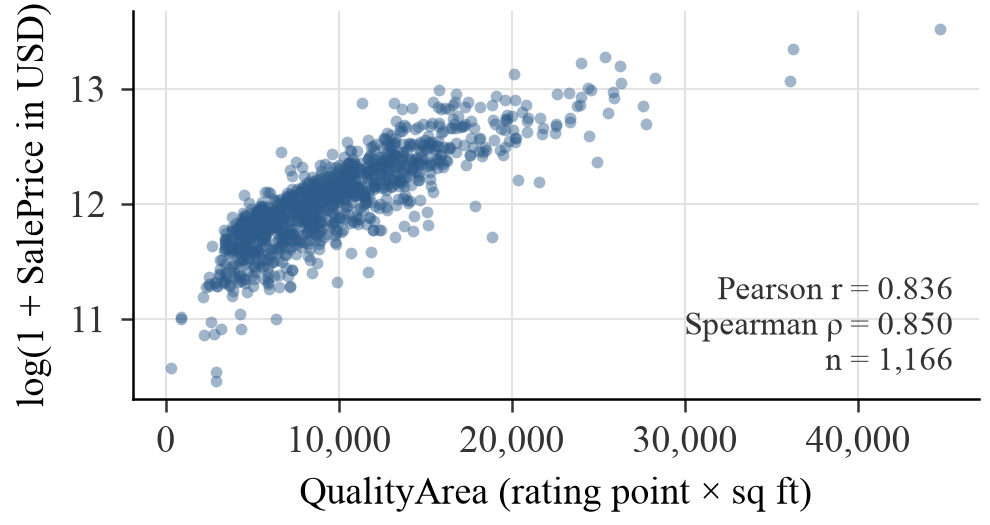
\includegraphics[width=\columnwidth]{figures/eda_qualityarea.png}
\caption{QualityArea (OverallQual $\times$ GrLivArea) against log sale price on the training data ($n = 1{,}166$), the evidence behind H1; its predictive gain is tested in \S\ref{sec:results}.}
\label{fig:eda}
\end{figure}
             % W2  §4
% Budget: ~1.5 columns  |  13 pts.  Slides p.10-11.
% Sources: results/README.md (I2), model/report/P3_model_choice_and_results.md,
%          model/results/tables/model_choice/model_choice_evidence.csv (P3).
\section{Method}
\label{sec:method}

\begin{figure*}[t]
\centering
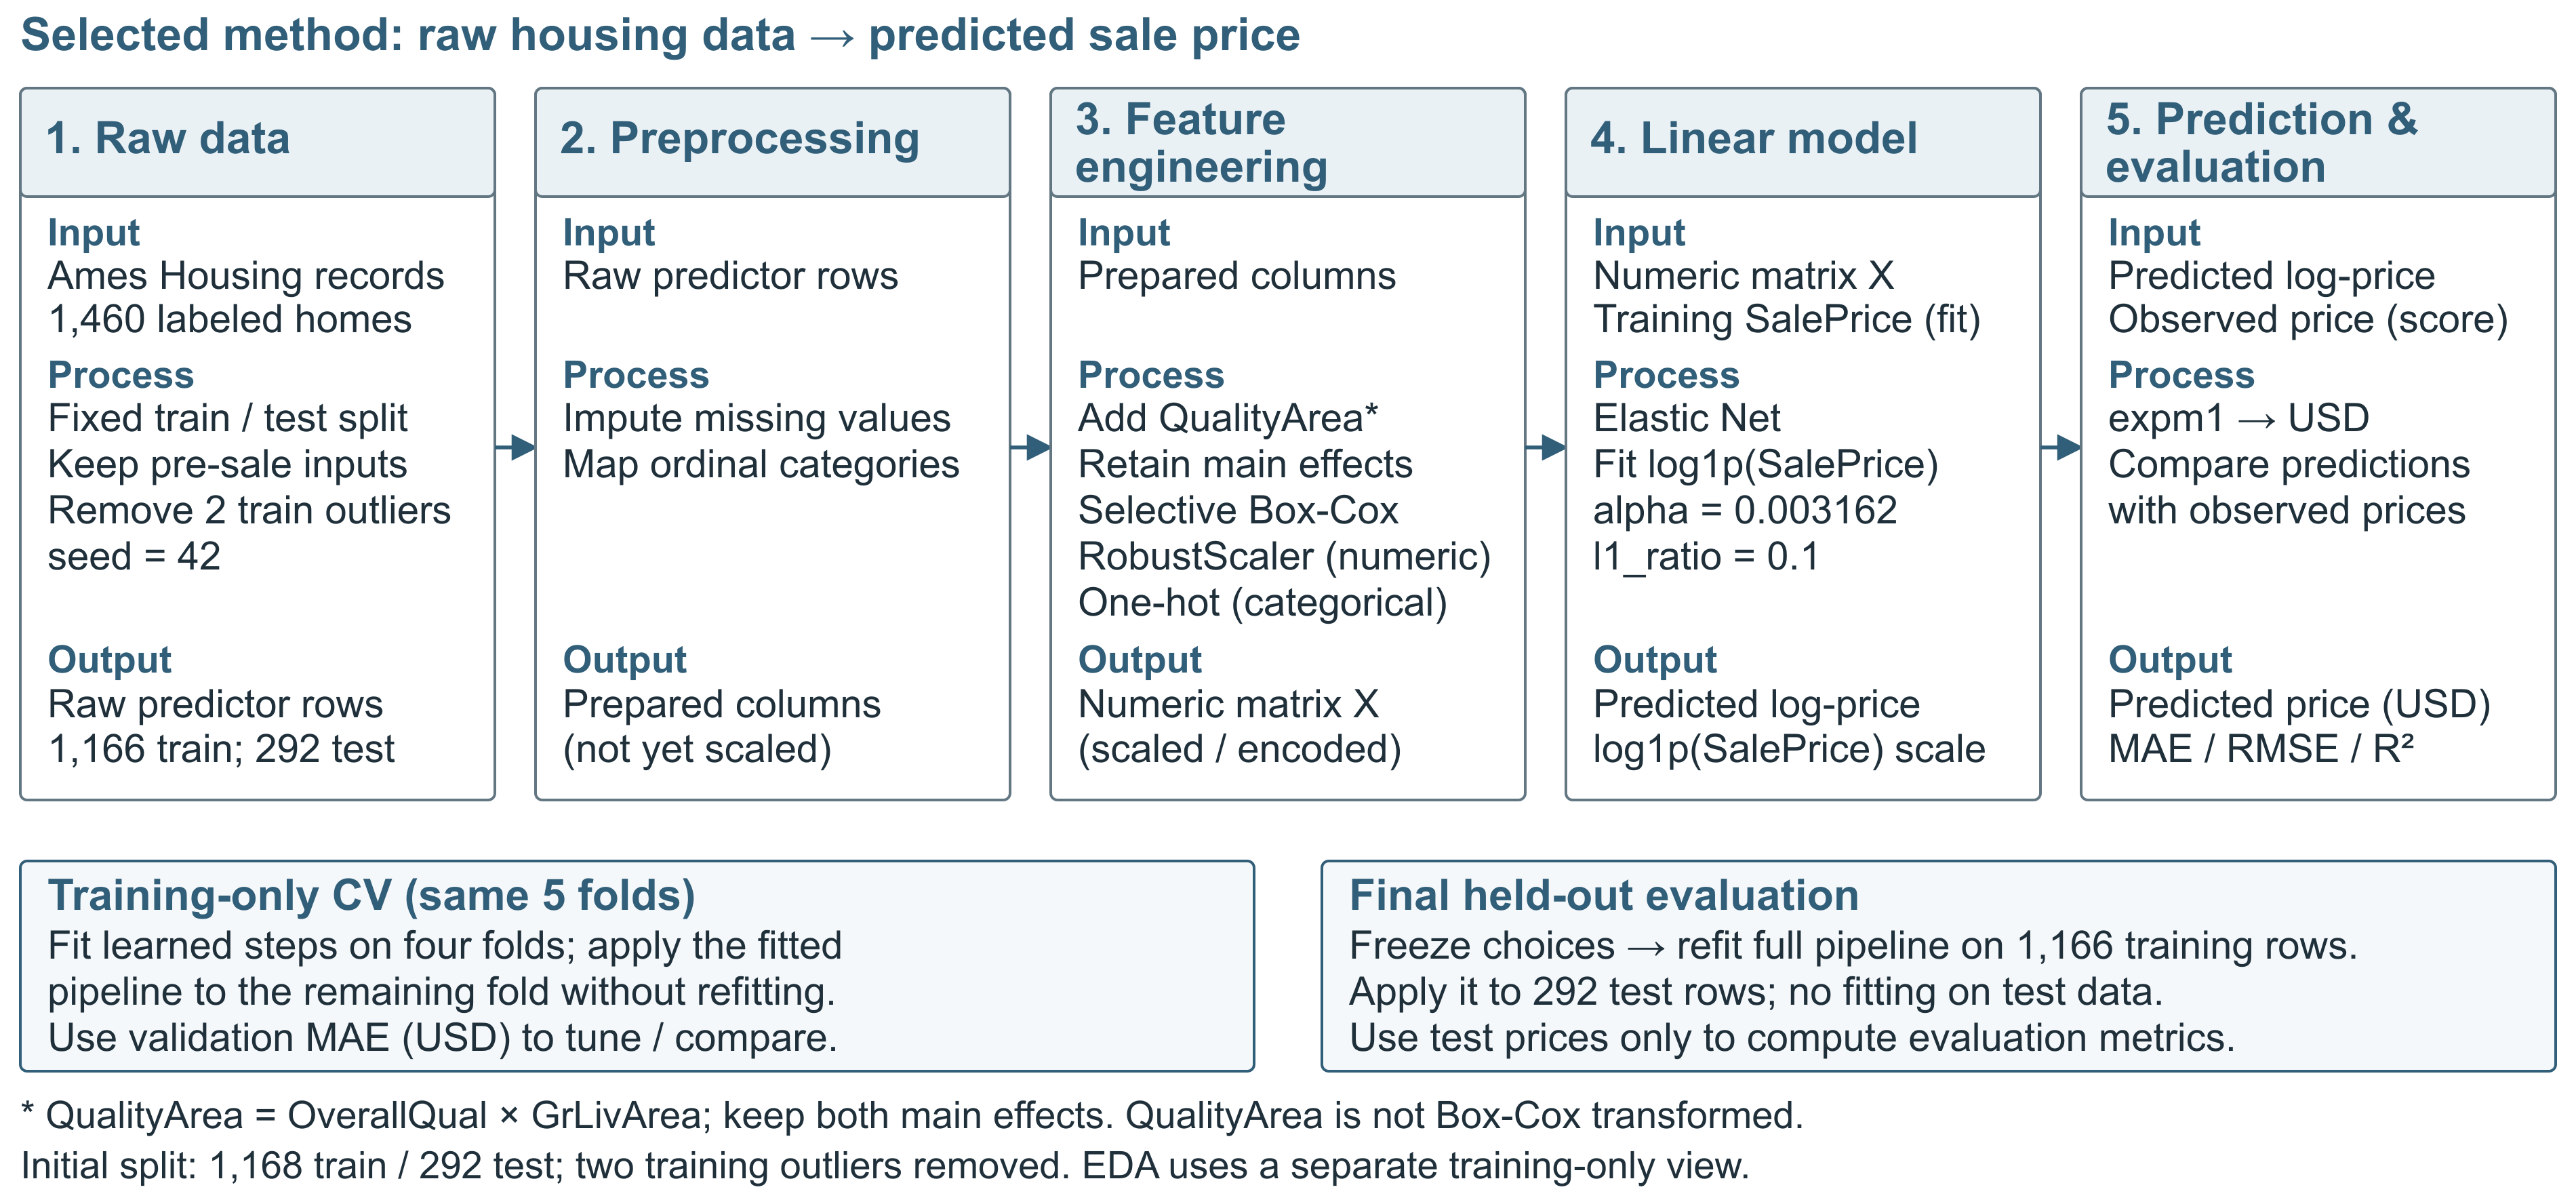
\includegraphics[width=0.95\textwidth]{figures/pipeline.png}
\caption{Five-stage pipeline from raw records to predicted sale prices, with each stage's input, processing and output. Learned steps are fitted within each training fold only; after all choices are frozen, the pipeline is refitted on 1,166 training rows and applied once to 292 test rows.}
\label{fig:pipeline}
\end{figure*}

\subsection{Pipeline and Feature Engineering}
Figure~\ref{fig:pipeline} shows the full pipeline. We designed one feature group per hypothesis.
\textbf{Interaction (H1):} QualityArea lets a linear model give each square foot a value that rises with quality; both main effects are kept.
\textbf{Transform (H2):} LogLotArea captures diminishing returns to land.
\textbf{Aggregate (H3):} TotalSF summarizes floor area in one column.
Only QualityArea is used in the final model (\S\ref{sec:results}).

\subsection{Model Choice and Hyperparameter Tuning}
The data have strongly correlated attribute groups and over 200 encoded predictors, many of them weak.
OLS is unstable here: its coefficients are not unique under rank deficiency, and it is our weakest linear model (CV MAE 14{,}958~USD).
Ridge \citep{hoerl1970ridge} handles collinearity but keeps all 209.8 predictors on average.
Lasso \citep{tibshirani1996lasso} removes weak predictors, but within a correlated group it tends to keep one member arbitrarily.
We therefore use Elastic Net \citep{zou2005elastic}, which combines both penalties and keeps 113.4 non-zero coefficients on average.
Its standardized coefficients are also stable across folds (mean pairwise cosine 0.960 vs.\ 0.954 for Lasso).
Its CV MAE ties with Lasso's (13{,}366 vs.\ 13{,}361~USD, a gap far below the fold SD of about 800~USD), so the choice rests on data structure rather than on the score.

We tune by grid search on the five training folds, minimizing MAE in USD.
The ranges are $\alpha \in [10^{-5}, 1]$ (11 log-spaced values) for Lasso and Elastic Net, with L1 ratio $\in \{0.1, 0.5, 0.9\}$ for the latter, and $\alpha \in [10^{-3}, 10^4]$ (15 values) for Ridge.
The selected Elastic Net uses $\alpha = 0.00316$ and an L1 ratio of 0.1, i.e., mostly L2 shrinkage with modest sparsity.
          % W2  §5
% Budget: ~1 column  |  10 pts.  Slides p.12-13.
% Sources: data/README.md (P1), research_story/README.md (I1), model notebooks (P3).
\section{Experimental Setup}
\label{sec:setup}

\subsection{Validation Protocol}
The 292 test sales are held out from the start and used once, after the features, model, hyperparameters and threshold are frozen.
The 1{,}166 training sales form 5 fixed folds (233/234/234/232/233 rows) shared by every method; each row is a distinct sale predicted at the property level, not a time series, so we use plain K-fold rather than a grouped or temporal split.
Five folds keep about 930 rows for fitting and over 230 per validation fold; we report mean $\pm$ SD.

\subsection{Metrics and Baselines}
\textbf{Metrics.} MAE in USD is the primary metric, because it is the typical size of a pricing mistake a seller or buyer faces.
RMSE in USD emphasizes large misses, which are costly in a negotiation.
$R^2$ shows the share of price variance explained.

\textbf{Decision threshold.} A model is usable if its MAE is at most 15{,}000~USD, fixed before testing, for two reasons.
For users, it is about 9\% of the median training price, accurate enough for a first asking-price estimate but not a substitute for a formal appraisal.
For generalization, it is the final model's CV MAE plus two fold SDs ($13{,}366 + 2 \times 809 = 14{,}985$~USD), rounded up, so a higher test MAE would signal worse performance than normal fold variation.
All three baselines exceed it in CV, so it separates usable from unusable models.

\textbf{Baselines.} (i)~\emph{Trivial:} the training-set mean price.
(ii)~\emph{Simple:} OLS on living area alone, the most intuitive single feature.
(iii)~\emph{Strong:} a Random Forest (300 trees) on the raw features and raw price, tuned over maximum depth $\{\text{none}, 10\}$, minimum leaf size $\{1, 3\}$ and feature fraction $\{0.7, 1.0\}$.
We also tried the log target for the forest; it was worse (CV MAE 16{,}800 vs.\ 16{,}554~USD), so we keep the raw price.
     % W2  §6
% Owner: W2  |  Budget: ~1.75 columns  |  18 pts
% Sources: results/tables/02_model_comparison.md, 03_feature_ablation.md (I2)
\section{Results}
\label{sec:results}

\begin{table*}[t]
\centering
\footnotesize
\begin{tabular}{@{}l r r r r r@{}}
\toprule
\textbf{Model} & \textbf{CV MAE} & \textbf{CV RMSE} & \textbf{Test MAE} & \textbf{Test RMSE} & \textbf{Test $R^2$} \\
\midrule
Training mean              & 56{,}392 $\pm$ 1{,}244 & 77{,}190 $\pm$ 4{,}334 & 62{,}580 & 87{,}620 & $-0.001$ \\
Single-feature OLS (GrLivArea) & 37{,}160 $\pm$ 2{,}295 & 53{,}092 $\pm$ 2{,}645 & 38{,}474 & 57{,}594 & 0.568 \\
Random Forest (raw)        & 16{,}554 $\pm$ 958     & 26{,}107 $\pm$ 2{,}431 & 16{,}384 & 27{,}018 & 0.905 \\
\textbf{Elastic Net + QualityArea} & \textbf{13{,}366 $\pm$ 809} & \textbf{19{,}925 $\pm$ 2{,}274} & \textbf{14{,}423} & \textbf{22{,}340} & \textbf{0.935} \\
\bottomrule
\end{tabular}
\caption{Main results. Errors in USD. CV: mean $\pm$ SD over the same 5 folds; Test: 292 held-out houses, evaluated once. Only Elastic Net meets the 15{,}000~USD MAE threshold.}
\label{tab:main}
\end{table*}

\subsection{Main Results}
% Slides p.14 (8%): every method; best per column in bold; compare against the
% threshold; why we win/lose vs the strong baseline; name the significance test.
% Caution (I2): same-feature Lasso CV MAE = 13,361 -- do not claim EN beats all
% candidates; CV was also used for tuning (not nested CV).
Under the same folds and test set (Table~\ref{tab:main}), only the Elastic Net meets the 15{,}000~USD threshold, with a test MAE of 14{,}423~USD.
This is within two fold SDs of its CV MAE; the Random Forest misses the threshold (16{,}384~USD).
The Elastic Net's per-house absolute error is 1{,}961~USD lower (paired bootstrap over test houses, 5{,}000 resamples: 95\% CI $[-3{,}847, -399]$; paired permutation test, 10{,}000 permutations: $p = 0.017$).
The gain is small but holds in every size and quality slice of the test set, most for large homes (23{,}372 vs.\ 27{,}316~USD MAE).

Two reasons likely explain the win.
First, with 1{,}166 sales and over 200 predictors, the data are too small for a forest to learn smooth size and quality effects, while log price is close to linear in them (Figure~\ref{fig:eda}).
Second, trees cannot extrapolate, which hurts most for the largest and most expensive homes.
Lasso ties in CV (\S\ref{sec:method}), so we do not claim the Elastic Net beats every linear variant.

\subsection{Feature Ablation}
% Slides p.15 (10%): same model, split and tuning; only the feature set changes.
% Set A raw, Set B top-k (inside each fold; justify k), Set C ours. Beat A and B
% by more than fold-to-fold variation? Slices
% (model/results/tables/final_test/slice_metrics.csv). Worth the cost?
Table~\ref{tab:ablation}(a) changes only the feature set, with the same model family, folds and tuning grid.
Adding QualityArea to the raw features (Set C) lowers CV MAE from 13{,}750 to 13{,}366~USD and CV RMSE by 6.8\%.
The MAE gain is smaller than one fold SD, but RMSE drops in all five folds, both here and under the controlled Ridge test (b), so the interaction mainly fixes large errors.
Slicing the out-of-fold predictions shows where: QualityArea lowers RMSE by 11.5\% for the largest third of homes by living area and by 13.7\% for OverallQual $\geq 8$ ($n = 182$), but changes it by at most 2.1\% elsewhere, as expected for a quality $\times$ size interaction.
Ranking features does not work: the MI top-20 set (Set B, re-selected inside each fold; $k = 20$ keeps the strongest quarter of the 73 candidates) is 3{,}600~USD worse in MAE than Set C, and $k = 15$ is worse still.
Adding the three engineered features to it cuts RMSE by 11\% but still trails Set A by 5\%: selection discards information the features cannot restore.

Table~\ref{tab:ablation}(b) tests each hypothesis with a fixed Ridge model.
H1 is supported: RMSE falls by 5.7\%, in all five folds.
H2 helps relative to raw lot area ($-1.1\%$) but adds nothing beyond the Box-Cox transform already in the pipeline.
H3 reduces three columns to one at a 1.1\% RMSE gain, within our 2\% tolerance.
We keep only QualityArea, because H2 and H3 change the error by about 1\%, well inside fold-to-fold variation; all three cost nothing to compute.

\begin{table}[t]
\centering
\small
\setlength{\tabcolsep}{4pt}
\begin{tabular}{@{}l r r@{}}
\toprule
\multicolumn{3}{@{}l}{\textit{(a) Elastic Net, tuned per set}} \\
\textbf{Feature set} & \textbf{CV MAE} & \textbf{CV RMSE} \\
\midrule
A: Raw                  & 13{,}750 $\pm$ 827   & 21{,}376 $\pm$ 3{,}271 \\
B: MI top-20            & 16{,}966 $\pm$ 1{,}269 & 25{,}286 $\pm$ 2{,}906 \\
C: Raw + QualityArea    & \textbf{13{,}366 $\pm$ 809} & \textbf{19{,}925 $\pm$ 2{,}274} \\
\midrule
\multicolumn{3}{@{}l}{\textit{(b) Hypotheses, Ridge ($\alpha = 10$)}} \\
\textbf{Change} & \textbf{$\Delta$RMSE} & \textbf{Folds improved} \\
\midrule
H1: + QualityArea               & $-1{,}222$ & 5/5 \\
H2: LotArea $\rightarrow$ log   & $-241$     & 4/5 \\
H2: Box-Cox $\rightarrow$ log   & $-2$       & 3/5 \\
H3: 3 areas $\rightarrow$ TotalSF & $-235$   & 3/5 \\
\bottomrule
\end{tabular}
\caption{Feature ablation on the same 5 folds (USD). (b) Negative $\Delta$RMSE is an improvement; fold counts are descriptive, not significance tests.}
\label{tab:ablation}
\end{table}
         % W2  §7
% Owner: W2  |  Budget: ~1.75 columns  |  16 pts
% Sources: results/tables/04_coefficients.md, 05_error_cases.md (I2)
\section{Analysis}
\label{sec:analysis}

\subsection{Coefficients and Statistical Significance}
% Slides p.16 (8%): standardized coefficients with 95% CI, p-value (name the
% test), VIF; check signs against §4; explain reversals; practical significance
% in target units. Slides ask for EVERY feature: Figure (forest plot) shows all 55
% numeric/ordinal predictors; the 159 one-hot columns are summarized in the text
% and listed in full on GitHub. Figure script: figures/plot_coef_forest.py
% CAUTION: after Holm correction no coefficient is significant (min 0.214);
% 29 of 214 have a 95% CI excluding 0 only WITHOUT correction; 159 VIFs are inf.
Figure~\ref{fig:coef} shows every numeric and ordinal predictor of the final model (55 of 214 columns) with its standardized coefficient, bootstrap 95\% CI and $p$-value (1{,}000 training resamples, pipeline fixed), and VIF.
The 159 one-hot columns of the 19 nominal features are small: none exceeds $|\beta| = 0.019$ (poured-concrete foundation), a quarter of QualityArea's.
The seven largest coefficients are all positive; only OverallCond reverses its training correlation ($r = -0.03$).
Older houses carry higher condition ratings ($r = -0.39$ with YearBuilt), so that correlation mixes age with condition; at a fixed construction year, better condition goes with a higher price.
QualityArea has the largest effect, supporting H1: a one-SD increase goes with about 8\% higher price, or roughly 13{,}000~USD at the median price.
Living area and construction year follow at about 7\% (12{,}000~USD) each, and lot area adds about 4\% (6{,}400~USD), all practically meaningful next to the 15{,}000~USD threshold.

Collinearity matters: QualityArea, GrLivArea and OverallQual share information (VIF 33, 58 and 12).
The second-floor area is shrunk to exactly zero, because living area already contains it (VIF 67).
All 159 one-hot columns have infinite VIF, because each full set of dummies sums to one.
Only 29 of the 214 coefficients have a 95\% CI excluding zero.
None passes a Holm correction, but only because 1{,}000 resamples cannot give $p < 0.001$, which bounds the corrected $p$ at 0.214 over 214 tests.
We read the coefficients as associations, not causal effects.

\begin{figure}[t]
\centering
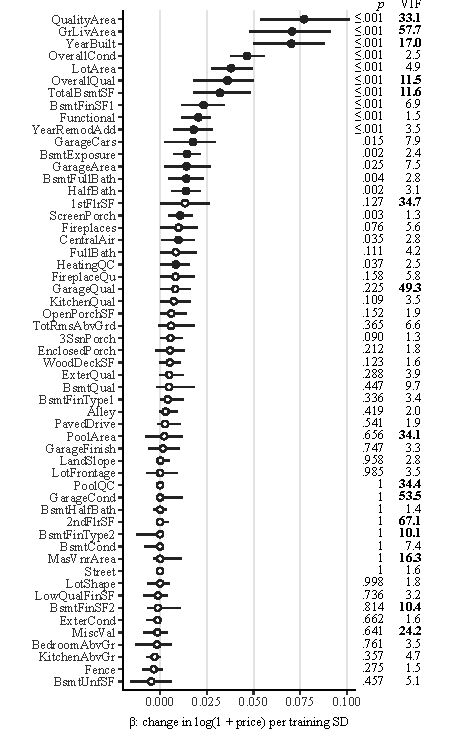
\includegraphics[width=\columnwidth]{figures/coef_forest.pdf}
\caption{All 55 numeric and ordinal coefficients with bootstrap 95\% CIs. Filled: CI excludes 0; $p$: uncorrected bootstrap; bold: VIF $\geq 10$. All 214 columns: \texttt{results/tables/04\_coefficients.md}.}
\label{fig:coef}
\end{figure}

\subsection{Error Analysis}
% Slides p.17 (8%): >= 3 largest-error test cases with actual, predicted, error
% (USD) and context; explain each; shared pattern and the first fix.
% Possible extra pattern (W1 check, discuss with P3/I1 before using): 6 of the 10
% largest errors, incl. all top 3, are SaleCondition = Partial (homes sold before
% completion) vs 9.2% of the test set; sale condition was excluded as a feature.
The three largest test errors (Table~\ref{tab:errors}) are all high-quality homes (OverallQual 8--9) in two of the three most expensive neighborhoods, underpredicted by 17--25\%.
Size alone does not explain this: house 775 is the smallest of the three but has the largest relative error.

The shared pattern: all three were new homes, built one year or less before the sale and sold before completion (sale type ``New'', sale condition ``Partial'').
Four of the ten largest errors are underpredicted new homes of this kind (Ids 899, 775, 1047 and 1244), although homes sold before completion are only 27 of the 292 test sales (9.2\%).
A fifth (Id 582) is overpredicted, so new construction adds error in both directions.
Without the sale year and sale type, the model cannot tell that these houses were brand new when sold.
The quality slices show the same effect: MAE rises from 11{,}085~USD for OverallQual $\leq 5$ to 27{,}636~USD for $\geq 8$ ($n = 45$).
The first fix is better input, not a bigger model: whether a house is newly built can come from building permits or the listing rather than the sale record, so a new-construction flag would respect our pre-sale rule.

\begin{table}[t]
\centering
\small
\setlength{\tabcolsep}{3.5pt}
\begin{tabular}{@{}r r r r l@{}}
\toprule
\textbf{Id} & \textbf{Actual} & \textbf{Pred.} & \textbf{Error} & \textbf{Context} \\
\midrule
899  & 611{,}657 & 473{,}938 & 137{,}719 & Q9, 2{,}364 ft$^2$, NridgHt \\
775  & 395{,}000 & 295{,}840 & 99{,}160  & Q8, 1{,}973 ft$^2$, NridgHt \\
1047 & 556{,}581 & 459{,}516 & 97{,}065  & Q9, 2{,}868 ft$^2$, StoneBr \\
\bottomrule
\end{tabular}
\caption{Largest absolute test errors of the final model (USD; error = actual $-$ predicted, so positive means underprediction). Q: OverallQual; area: GrLivArea.}
\label{tab:errors}
\end{table}
        % W2  §8
% Owner: W1  |  Budget: ~0.5--0.75 column  |  5 pts
% Slides p.18. Conclusion: answer the RQ with key numbers; which features
% mattered and why; one actionable recommendation; NO new results.
% Limitations: coverage; linearity/extrapolation; threshold assumptions; next experiment.
% Numbers: results/Results_Master.xlsx (I2).
\section{Conclusion and Limitations}
\label{sec:conclusion}

\paragraph{Conclusion.}
Our answer to the research question is yes: using only pre-sale attributes, the Elastic Net reaches a test MAE of 14{,}423~USD, within the 15{,}000~USD threshold, consistent with its CV MAE (13{,}366 $\pm$ 809~USD) and 1{,}961~USD below the Random Forest ($p = 0.017$).
The quality $\times$ living-area interaction mattered most, because space is worth more in a better-built house; with living area and construction year it carries the largest coefficients, while a correlation ranking alone (top-20 features) hurt accuracy.
Sellers and agents can use the model as a starting point for typical homes, but for high-quality and newly built homes (MAE 27{,}636~USD for OverallQual $\geq$ 8) they should allow a wider margin and seek a formal appraisal.

\paragraph{Limitations.}
The data cover one city in 2006--2010 (1{,}458 sales) and may not transfer to other markets or periods.
The model underpredicts high-end homes and should not be used beyond the observed size and quality range.
The threshold bounds the average error only: individual errors reach 137{,}719~USD, and its value rests partly on the final model's own cross-validation.
CV errors are slightly optimistic because the same folds were used for tuning.
As a next step, we would add a listing-time new-construction flag (\S\ref{sec:analysis}) and test whether it closes the gap for high-end new homes.
      % W1  §9 Conclusion & Limitations
% Owner: I3 collects; every member checks their own line.  |  counts toward the 6 pages  |  3 pts
% Slides p.19: one bullet per member naming concrete tasks and the sections or
% figures produced; AI usage statement (tools, steps, which decisions the team
% made and verified). Placed BEFORE the references.
% TODO: map each name to a role, and drop the member who left the group.
\section*{Contributions of Each Member}
\begin{itemize}
  \item \zh{李宗穎}: data source check, preprocessing, train/test split and CV folds (\S\ref{sec:data}).
  \item \zh{張翊鞍}: EDA, hypotheses H1--H3, feature definitions (\S\ref{sec:eda}, Figure~\ref{fig:eda}).
  \item \zh{范}\zhalt{瀞}\zh{予}: models, tuning, ablation, final test, significance and coefficient analysis (\S\ref{sec:method}--\S\ref{sec:analysis}).
  \item \zh{劉嘉豪}: application scenario, research question, decision threshold, storyline.
  \item \zh{周懷聖}: Results Master Sheet, final figures and tables (Figure~\ref{fig:pipeline}).
  \item \zh{陳家祥}: slides, repository, submission.
  \item \zh{陳柏淮}: literature review (\S\ref{sec:related}); wrote the paper from the team's results; oral presentation.
\end{itemize}

\paragraph{AI Usage Statement.}
We used Claude (Anthropic) to find and verify related work and to draft and format the paper from our result files, and ChatGPT and Codex (OpenAI) to organize result files and tables.
Members also used these tools for coding help and proofreading.
The team chose the task, features, models and threshold, ran all experiments, and verified every reported number against the result files.
   % I3  (counts toward the 6 pages)

\bibliography{references}

\end{document}
